\documentclass{config/apuntes}

\title{Transcriptómica, Regulación Genómica y Epigenómica}
\author{Sandra Mingo Ramírez}
\date{2024/25}
\acronym{TRREP}

\usepackage[all]{nowidow}
\usepackage{listing}
\usepackage{color}
\usepackage{tabularx}
\usepackage{multirow}
\usepackage{makecell}
\usepackage{amsmath}
\usepackage{array}
\usepackage{soul}

\definecolor{dkgreen}{rgb}{0,0.6,0}
\definecolor{gray}{rgb}{0.5,0.5,0.5}
\definecolor{mauve}{rgb}{0.58,0,0.82}

\lstset{
  frame=tb,
  aboveskip=3mm,
  belowskip=3mm,
  showstringspaces=false,
  columns=flexible,
  basicstyle={\small\ttfamily},
  numbers=none,
  numberstyle=\tiny\color{gray},
  keywordstyle=\color{blue},
  commentstyle=\color{dkgreen},
  stringstyle=\color{mauve},
  breaklines=true,
  breakatwhitespace=true,
  tabsize=3
}

\usepackage{tocloft}

\advance\cftchapnumwidth 0.9em\relax
\advance\cftsecnumwidth 0.6em\relax
\advance\cftsubsecindent 0.5em\relax
\advance\cftsubsecnumwidth 0.5em\relax
\begin{document}

\begin{abstract}
La asignatura aborda el análisis de datos de transcriptómica y proteómica, analizando las tecnologías disponibles, la cuantificación de la expresión y métodos para el análisis estadístico de la expresión diferencial. Además, se verán métodos de análisis funcional, estudios de la regulación genómica y epigenómica, análisis multimodal de datos de célula única y métodos de clasificación supervisada y no supervisada (clustering) aplicados a datos ómicos de bulk y de célula única.

Obtendremos la capacidad de analizar de manera cuantitativa datos de transcriptómica y proteómica tanto a nivel de tejido como de célula única, e integrarlo con técnicas para el estudio de la expresión de la transcripción, tales como la modificación de histonas y la actividad de la cromatina y los factores de transcripción.
\end{abstract}

\pagestyle{plain}

\maketitle

\tableofcontents

%Examen tipo test sin restar 50% 
%2 trabajos 40%
%Participación 10%

%29/01 - Fátima Sánchez Cabo
\chapter{Diseño experimental y principios estadísticos del análisis de datos ómicos}
El transcriptoma permite estudiar cómo se expresan los ARNs. Después va el proteoma, el cual se centra en el estudio de las proteínas. El último paso es el del metaboloma. Genómica, transcriptómica y proteómica se pueden analizar con NGS y arrays, mientras que proteómica y metabolómica se estudia con espectometría de masas. Para la proteómica, aunque la espectometría de masas tiene mayor detalle, la secuenciación es más escalable, por lo que se está popularizando. Concretamente hay dos casas comerciales que lo permiten: Olink y Somalogic. 

\section{Pipeline de un experimento ómico}
Esto aplica a la cuantificación de la expresión con NGS, con espectometría de masas o de metabolitos con espectometría. La primera parte es la pregunta biológica. Un experimento de ómicas se basa en una pregunta clara de qué es lo que se busca en los datos. 
Esta pregunta guía la plataforma a utilizar. Por ejemplo, la proteómica se puede estudiar por secuenciación o por espectometría. Si tenemos una cohorte humana grande y queremos datos abundantes, quizás la mejor opción puede ser la secuenciación. En general, la tecnología nunca debe guiar, se debe elegir en función de la pregunta. Después hay que definir el diseño experimental. Una vez hecho el experimento, se analiza la imagen, se preprocesan los datos, se normalizan y se analizan. Dentro del análisis de datos, dentro de las ómicas para la cuantificación tienen tres pasos importantes: identificación de genes diferencialmente expresados, análisis de cluster y métodos de ingeniería reversa. Tras esto, se estandariza y se guardan los datos y finalmente se integran los datos y se interpreta biológicamente. Una base de datos importante es la base de datos GEO, Gene Expression Omnibus. 

\section{Diseño experimental}
Esta parte es esencial, ya que los experimentos son muy caros. Se trata de utilizar ciertos principios para que el coste sea el menor posible, y a la vez poder extraer toda la información posible con ese coste. En otras palabras: minimizar el coste y maximizar la información obtenida.

Para hacer un buen diseño experimental, hay dos cosas esenciales:
\begin{enumerate}
\item \textbf{Pregunta biológica:} es imprescindible saber qué se está buscando para generar un experimento; ver si es data-driven o hypothesis-driven.
\item \textbf{Conocimiento de la tecnología:} medidas robustas y precisas de los datos. Replicación, tipo de variables que pueden meter sesgos en el experimento o variabilidad técnica. Estas técnicas buscan ser cuantitativas. 
\end{enumerate}

En un experimento, hay dos tipos de errores:
\begin{itemize}
\item \textbf{Errores aleatorios:} no son posibles de calibrar, pero se minimizan mediante la repetición de las mediciones.
\item \textbf{Errores sistemáticos:} es posible de estimar y de eliminar de los datos. También se reduce normalizando, ya que son problemas de calibración.
\end{itemize}

A través de tres principios, se busca eliminar estos errores: replicación, randomización y blocking.

La distinción entre réplicas biológicas y técnicas depende de qué fuentes de variación se estudien o, alternativamente, se consideren fuentes de ruido. Existen las réplicas técnicas, las cuales minimizan los errores aleatorios mediante el promedio y ayudan a testar la tecnología, y réplicas biológicas, que permiten sacar conclusiones extrapolables a la población completa y no solo del individuo, además de poder controlar la variabilidad en diferentes pasos experimentales.

Supongamos que se realiza un experimento en el que se puede medir la expresión de un gen en una sola célula y se dispone de dinero para realizar 48 mediciones. Tenemos varias repeticiones: utilizamos varios ratones (replicación biológica), de cada ratón escogemos varias células (replicación técnica/biológica, está entre medias), y se realizan varias medidas dentro de cada célula (replicación técnica). Las medidas de la misma célula deberían ser muy parecidas. Si se realiza la media de los tres ratones, la medida va a ser muy variable en relación con una sola medida, pero esto sirve para el test estadístico, ya que son medidas independientes. En caso de tener medidas dependientes, no se puede utilizar la variabilidad para estudiar la significancia, ya que son medidas repetidas. 

En el modelo propuesto hay que cuantificar bien la variabilidad. ¿Cómo escoger el tipo y número de réplicas? En un experimento de ómicas en el que se mide la expresión de un gen de células de hígado de ratón, se cuantifica una expresión de 12. Se realizan dos tipos de variabilidad biológica (animal y célula) y una variabilidad técnica (medición). Estas tres fuentes de variabilidad suman un 3,5 de variabilidad. Las normales están centradas en 10, ya que las medidas están saliendo en ese valor, no en 12. Hay más variabilidad biológica que técnica, transformando las gaussianas en una parábola más aplastada. Se realizaron simulaciones cambiando el número de animales, el número de células y el número de réplicas técnicas. Se hacen 10.000 asignaciones, para que se agrupen de forma diferente las combinaciones del número total (48 animales, 1 sola célula; 24 animales, 2 células; ...; 1 animal, 48 células). Sabiendo la cantidad de animales, células y mediciones, se puede sacar el tamaño muestral real del experimento, permitiendo calcular así la diferencia entre la variabilidad experimental y la variabilidad real. En ómicas, somos poco capaces de estimar la variabilidad, ya que en general hay pocas réplicas. Si esto después de mete en un t-test, y la variabilidad es muy pequeña (o incluso 0), entonces el resultado es muy grande, teniendo un p muy pequeño, rechanzando la hipótesis nula de que no hay diferencia en la expresión.

Para tecnologías ómicas, se deben incluir al menos 3 réplicas biológicas. Todo esto es para la experimentación con animales. En caso de experimentación en humanos, la variabilidad es gigante. 

Cuando comenzó la secuenciación, cuanto más se secuencie, más caro es el experimento. Por tanto, ¿es mejor más réplicas a menos profundidad, o menos réplicas a más profundidad? Hubo varios estudios con muchas simulaciones que vieron que lo importante era la secuenciación con réplica biológica. El número de lecturas tiene algo de relevancia, pero llegados a un número, no compensa a hacer mucha más secuenciación porque se llega a un plateau en cuanto a genes diferencialmente expresados. Las métricas aumentan más teniendo varias réplicas biológicas que teniendo varias lecturas. 

Una forma de incrementar el número de individuos manteniendo el coste bajo es mediante el \textbf{pooling} de muestras. En el caso de muestras humanas no se hace porque se pierde información fenotípica y genotípica importante del paciente, pero en animales sí puede ser una buena idea si las características específicas por especimen (sexo, camada, edad, etc.) no son relevantes para el experimento. Lo mejor es tener cuantas más réplicas independientes posibles. 

Algunos pasos en los que se introduce variabilidad en NGS son:
\begin{itemize}
\item Técnica: extracción del ARN, preparación de la librería, flow-cell, barcode, científico
\item Biológica: sexo, camada/familia, edad
\end{itemize}
Además, hay sesgos sistemáticos y ruido por errores aleatorios.

Cuando hay estudios muy grandes, hay pasos que se deben realizar en varias tandas. Al secuenciar en diferentes días, se introduce variabilidad. Esto se conoce como el \textbf{efecto de batch}. \marginpar[\footnotesize !!!!!]  \ Nunca hay que confundir el batch con el grupo biológico relevante, ya que es imposible ver si las diferencias son debidas al grupo biológico o a la variabilidad técnica. Cuando hay condiciones biológicas muy fuertes, a veces no se ven, pero si se hacen todas las muestras de una condición en un mismo batch, probablemente se estén magnificando las diferencias observadas. Por tanto, no hay que medir las distintas condiciones biológicas en batches distintos, si no mezclar en un batch muestras de distintas condiciones biológicas para poder utilizar la variable batch en el modelo estadístico mixto, normalizando por las diferencias entre los batches.
%SUPER IMPORTANTE EFECTO DE BATCH

El \textbf{blocking} reduce fuentes conocidas e irrelevantes de variación entre unidades, permitiendo una precisión mayor en la estimación de las fuentes de variación estudiadas. Minimiza el efecto de variables de tipo biológico o técnico, que no son relevantes para la pregunta biológica. Una forma de hacer blocking secuenciando es metiendo adaptadores para hacer un barcoding de cada muestra, preparar la librería con todo junto y crear, de esa muestra, las distintas alícuotas a secuenciar. De esta forma se reduce el efecto de línea.

Todo esto se basa también en la \textbf{randomización}, de forma que sea representativo de la población. 

\subsection{Diseño experimental - Ejercicios}
\subsubsection{Ejercicio de animales}
Tenemos un ratón knock-out en la proteína Bmi1. Para cada camada tenemos varios ratones WT y KO. Queremos encontrar metabolitos cuya expresión cambie significativamente entre condiciones
Disponemos de 6 camadas con el siguiente número de animales:
\begin{table}[h]
\centering
\begin{tabular}{c | c c}
Camada & KO & WT \\ \hline
L1 & 1 & 2 \\
L2 & 2 & 2 \\
L3 & 1 & 1 \\
L4 & 1 & 3 \\
L5 & 2 & 3 \\
L6 & 3 & 2 
\end{tabular}
\end{table}

\begin{itemize}
\item \textbf{Caso 1: No hay limitación económica}: se secuencia todo, ya que cuantas más muestras independientes, mejor.
\item \textbf{Caso 2: Se pueden secuenciar un máximo de 6 muestras}: De las 6 camadas se escogen aleatoriamente 3, de las cuales escoger un ratón KO y uno WT. Otra opción es coger las camadas 2 y 3 y secuenciar todos esos individuos. En este caso, como las camadas tienen efecto, se podría elegir un individuo de cada camada y hacer pool de 2 en 2. 
\item \textbf{Caso 3: L5 no tiene ningún animal KO y seguimos con el máximo de 6 muestras}: L5 no se tendría en cuenta porque podría introducir sesgos (quizás el KO no ha salido, o quizás no es viable), y del resto de camadas se escogen 3 camadas al azar para seleccionar un ratón de cada condición. Esto se debe a que no se podría comparar el pool entre la misma camada con pool entre distintas camadas.
\item \textbf{Caso 4: máximo de 6 muestras si no hay efecto de la camada}: se mezclan todos los ratones de las distintas camadas, separando por condición biológica, y se sacan 3 de cada uno al azar. Se podrían coger 12 y 12 y pooles de 4, o 6 y 6 y pooles de 2.
\end{itemize}

\subsubsection{Ejercicio de humanos}
Tenemos una cohorte de 100 muestras humanas con diabetes. Queremos probar en ellas un fármaco y ver sus efectos en la expresión génica. Podemos secuenciar un total de 40 muestras. Por estudios piloto sabemos que el sexo y el IMC afectan al impacto del fármaco. La composición de la cohorte es la siguiente:
\begin{table}[h]
\centering
\begin{tabular}{c | c c}
 & Hombres & Mujeres \\ \hline
IMC alto & 40 & 20 \\
IMC bajo & 20 & 20
\end{tabular}
\end{table}
Además, no podemos procesar todas las muestras juntas, tenemos que hacerlo en dos ejecuciones.
\begin{itemize}
\item \textbf{Q1: ¿Cómo se asignan los pacientes a los grupos fármaco y placebo?} Se escogen 5 personas de cada condición (sexo y BMI) para fármaco y otros 5 para placebo. 
\item \textbf{Q2: ¿Qué pacientes se secuenciarían en cada turno?} Se cogen ordenadamente una muestra de cada grupo y condición.
\end{itemize}

\section{Consideraciones estadísticas para datos ómicos}
%05/02 - Fátima Sánchez Cabo
\part{Transcriptómica}
\chapter{RNA-Seq}
\section{Pipeline general y alineadores}
En este curso nos centraremos en los NGS de lectura corta (segunda generación). Para transcriptómica, se secuencia el cDNA generado a partir del ARNm. Este cDNA se fragmenta y se secuencia en reads cortos. Las máquinas y la forma de secuenciar es la misma que aquella vista en la asignatura "Fundamentos de Secuenciación". 

Las lecturas pueden ser solo de la primera parte del fragmento (single-reads) o lecturas pareadas para tener una mayor precisión en el alineamiento. Del secuenciador sale un fichero FastQ, el cual se alinea con un genoma de referencia en FastA. Una vez con los alineamientos, se pueden mirar las regiones con reads mapeadas que estén en el transcriptoma de referencia (GTF/GFF) y cuantificar la expresión (matriz de conteo en CSV/TSV). 

En general, el workflow es el siguiente: descargar datos, QC inicial, pre-procesamiento y QC posterior, alineamiento a una referencia, detección, conteo y análisis estadístico. En transcriptómica, se quiere cuantificar la expresión de las partes del genoma que se transcriben. Por ello, se necesita un genoma de referencia, pero también otro archivo GTF que relacione los exones con los tránscritos y los genes. El contaje por detección es el que se hace con CHIP-Seq, al secuenciar la parte del ADN genómico a la que se ha pegado un factor de transcripción predefinido. 

\begin{figure}[h]
\centering
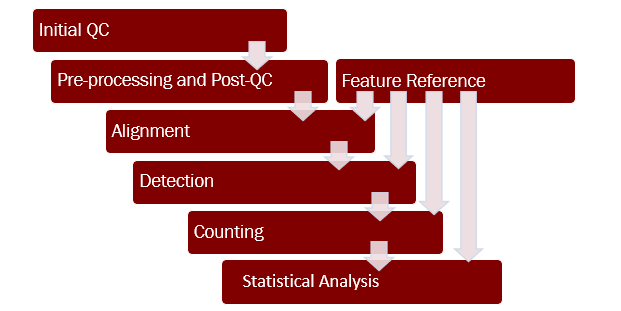
\includegraphics[width = 0.8\textwidth]{figs/ngs-analysis-workflow.png}
\end{figure}

\subsection{Control de calidad inicial}
Los objetivos del control de calidad de las lecturas crudas es detectar problemas de secuenciación, detectar adaptadores y comparar librerías para análisis posteriores. Distintos experimentos requieren interpretaciones distintas del análisis de control de calidad. Una herramienta muy utilizada para esto es FastQC. El análisis de la calidad por base, representa la distribución de las puntuaciones de calidad en todas las lecturas por la posición de cada lectura. En general, es normal que las últimas posiciones tengan una calidad algo peor que las demás, pero una buena muestra debe seguir teniendo una calidad alta. Si una muestra no tiene gran calidad, se puede optar por utilizar solo aquella porción de las muestras que tienen una calidad aceptable, pero hay que tener en cuenta que al acortar las lecturas, el mapeado puede darse en un mayor número de sitios. También se mide el contenido de cada base por posición (que debería ser bastante constante a lo largo de toda la lectura dependiendo de la "complejidad de la muestra", es decir, variedad de tránscritos diferentes) y la puntuación de calidad media por secuencia. La pipeline para el ARNm y los miRNA es la misma, pero hay peculiaridades. Los microARNs son ARNs de unos 20-30 nucleótidos que reprimen la expresión génica de los genes a los que se unen.
Dado el bajo número de miRNAs codificados por el genoma y el más reducido número expresado en cada tejido es de esperar ver perfiles de baja complejidad en las librerías de miRNAs, dádose así un patrón irregular del contenido de bases por posición.

Las secuencias sobrerrepresentadas son listas de secuencias que están presentes más veces de lo esperado por azar. La lista sobrerrepresentada se anota con el tipo de secuencia si se proporciona una lista con la que comparar. Normalmente, las secuencias adaptadoras pueden estar sobrerrepresentadas si hay altos niveles de ligaciones de dímeros de cebadores en el paso de preparación de la biblioteca. A menudo se debe a un desequilibrio entre los niveles de adaptadores y los niveles de fragmentos de muestra. Algunos RNA-Seq de tejidos particulares pueden dar también secuencias sobrerrepresentadas. Por ejemplo, las muestras de sangre contienen grandes cantidades de transcritos de hemoglobina que siempre se reportan como lecturas sobrerrepresentadas. Las muestras de miARN siempre muestran secuencias sobrerrepresentadas. Las bibliotecas de ARN total muestran secuencias sobrerrepresentadas de ARN ribosómicos.

\subsection{Preprocesado}
El preprocesado tiene como objetivo mejorar la calidad, la mapeabilidad, quitar contaminantes y sesgos, etc. Hay diferentes herramientas, como cutadapt o trim-galore. 

La calidad de las bases puede afectar al análisis de llamadas de variantes y, si es grave, también al mapeo de características. La calidad de las bases suele disminuir al final de la lectura y a veces al principio. Además, la secuenciación de baja calidad puede producir un grupo de lecturas de baja calidad a lo largo de su longitud. Es esencial eliminar las bases de baja calidad para el análisis de llamada de variantes. Para otros análisis, elimínelas sólo si afecta al rendimiento del mapeo.

\subsection{Alineamiento y mapeado}
Hay dos tipos de alineamientos: local y global. En el caso del local, se busca que en partes específicas el alineamiento sea bueno, mientras que en el global se busca meter la lectura en la secuencia completa, metiendo gaps. 

La cobertura en un segmento se mide como el número de reads que mapean a ese fragmento del genoma y la longitud de cada lectura dividido por la longitud del fragmento. Para poder hacer el mapeado se necesita la referencia en fasta, las reads en fastq y una referencia indexada. Esto es distinto de los alineadores tradicionales como BLAST. El objetivo es mapear las lecturas a las características. En transcriptómica, el alineamiento se realiza al mismo tiempo que la cuantificación. 

Lo importante es la indexación del genoma de referencia para ahorrar tiempo de computación. El genoma se corta en trozos para que sea más fácil realizar las búsquedas. Esto se puede hacer por ejemplo con BWA y alineadores Bowtie que utilizan la transformación de Burrows-Wheeler al ser más rápidos.

Aunque se hable de expresión génica, los genes no se expresan, son los tránscritos. Con estas técnicas es muy complicado hilar tan fino, por lo que se cuantifican los reads al gen y contar. A la hora de alinear, si se intenta alinear reads al genoma de referencia, las reads salen del tránscrito, por lo que puede ocurrir que una parte de un read caiga en un exón y la otra parte en el otro. Esto se puede visualizar con el visor IGV. Las lecturas partidas se conocen como \textbf{exon junctions}. Por ello, se puede mapear al genoma permitiendo esa característica. Otra opción es alinear directamente al transcriptoma, pero es más grande que el genoma (puede haber 100.000 tránscritos definidos vs 20.000 - 30.000 genes) y puede que haya lecturas que no se puedan mapear a un tránscrito concreto, si no que puedan mapear a varios tránscritos con el mismo exon.

\begin{figure}[h]
\centering
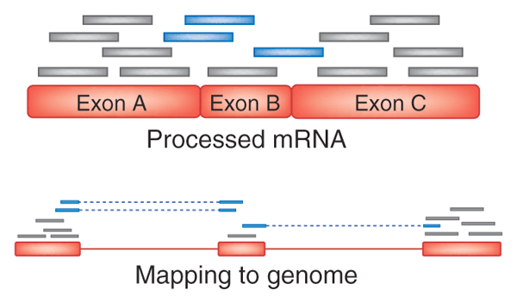
\includegraphics[width = 0.5\textwidth]{figs/Imagen1.png}
\end{figure}

\subsection{Galaxy}
Galaxy es una plataforma con muchas herramientas y workflows ya hechos para investigación biomédica intensiva en datos. Permite generar y hacer públicas pipelines. Se puede utilizar en el servidor europeo o montar un servidor local. 

Para nuestro proyecto, utilizaremos los datos del paper "Next-generation sequencing facilitates quantitative analysis of wild-type and Nrl(-/-) retinal transcriptomes". En la parte de "Related Information" se encuentran los datasets subidos a la base de datos GEO (Gene Expression Omnibus). En general, las revistas buenas exigen poner los datos en una base de datos pública. En este caso hay 6 muestras, 3 wild-type y 3 knock-out. Cada muestra en GEO tiene un ID. 

Galaxy se conecta a las bases de datos mediante API, por lo que se puede poner el link a los reads crudos y Galaxy lo lleva a nuestra sesión sin necesidad de descargarlos de las bases de datos y subirlos a Galaxy de forma manual. 

Nos vamos a descargar la información de los nombres de las muestras (los metadatos). Desde GEO, hay un acceso a SRA Run Selector donde tenemos disponibles esos datos. Hay dos tablas disponibles: metadata y lista de las accesiones con los IDs de las muestras. Los metadatos se necesita posteriormente para saber qué muestras son WT y cuáles KO, pero por ahora solo necesitamos los IDs para subir a Galaxy. El siguiente paso es decirle a Galaxy que, utilizando esos identificadores, se descarguen los FastQ. Para ello, en Get Data hay una opción de Faster Download and Extract Reads in FastQ format from NCBI SRA. Para esa herramienta se selecciona la opción de "List of SRA accessions, one per line" y se ejecuta.

Una vez con los datos, vemos que en Pair-end tenemos 0 datos y en Single-end 6, indicando que las muestras son single-end (aunque esto ya lo sabíamos porque venía en SRA Run Selector). El siguiente paso es ir a FastQC con los datos de single-end. La salida es un fichero txt con los números y un html con las imágenes. Tras analizarlo brevemente, vemos que no hay ningún problema con las muestras, pudiendo continuar con el análisis.

En Ensembl nos vamos a la página de FTP Downloads donde se encuentran todas las referencias de la última versión del genoma. Para reproducir unos resultados, hay que utilizar la referencia de la fecha de publicación de los datos que se estén utilizando, pero en nuestro caso podemos utilizar la última versión generada. Como no queremos descargar el Fasta a nuestro ordenador, vamos al FastA y buscamos el fichero de primary assembly. Con click derecho, podemos copiar el enlace y en Galaxy, en Upload, se puede utilizar la función Paste/Fetch data y pegar ahí la dirección. También subimos el GTF de los cromosomas.

%07/02 - Fátima
El siguiente paso es buscar la herramienta Trim-Galore con los datos single-end dejando todas las opciones como las predeterminadas. Con esta herramienta queremos quitar los adaptadores, y en caso de tener muestras dañadas, podríamos también eliminar esa parte. 

\section{Expresión diferencial}
\subsection{Visualización con IGV}
Para subir un fichero a IGV, nos vamos a File y Load from File. Hay que tener en la misma carpeta el fichero BAM con el fichero BAI, es decir, el fichero indexado. Hay que cargar el BAM. Se muestran tres tracks, siendo uno la cobertura, otro los junctions y el último los duplicados (click derecho y expandir). Previamente hay que seleccionar el genoma correcto; en este caso, el de ratón. 

Podemos irnos al cromosoma 13 y buscar el gen Smn1, con eso saltamos a esa región del genoma. Podemos ver las distintas isoformas del gen y dónde han mapeado las lecturas. En Junctions, vemos que hay lecturas con un arco grande, indicando que la lectura ha mapeado a esos exones que estaban juntos en el tránscrito, pese a que en el genoma estén separados por intrones y otras regiones no codificantes. La cobertura coincide con los exones al tratarse de un RNA-Seq. Además, tiene una cobertura 0-20, indicando que en ese rango hay como máximo 20 reads y como mínimo 0. 

La isoforma superior tiene un exón al principio de la proteína que no tiene ninguna lectura. Esto puede darse por la cobertura baja, indicando que nos estamos perdiendo esa isoforma.

\begin{figure}[h]
\centering
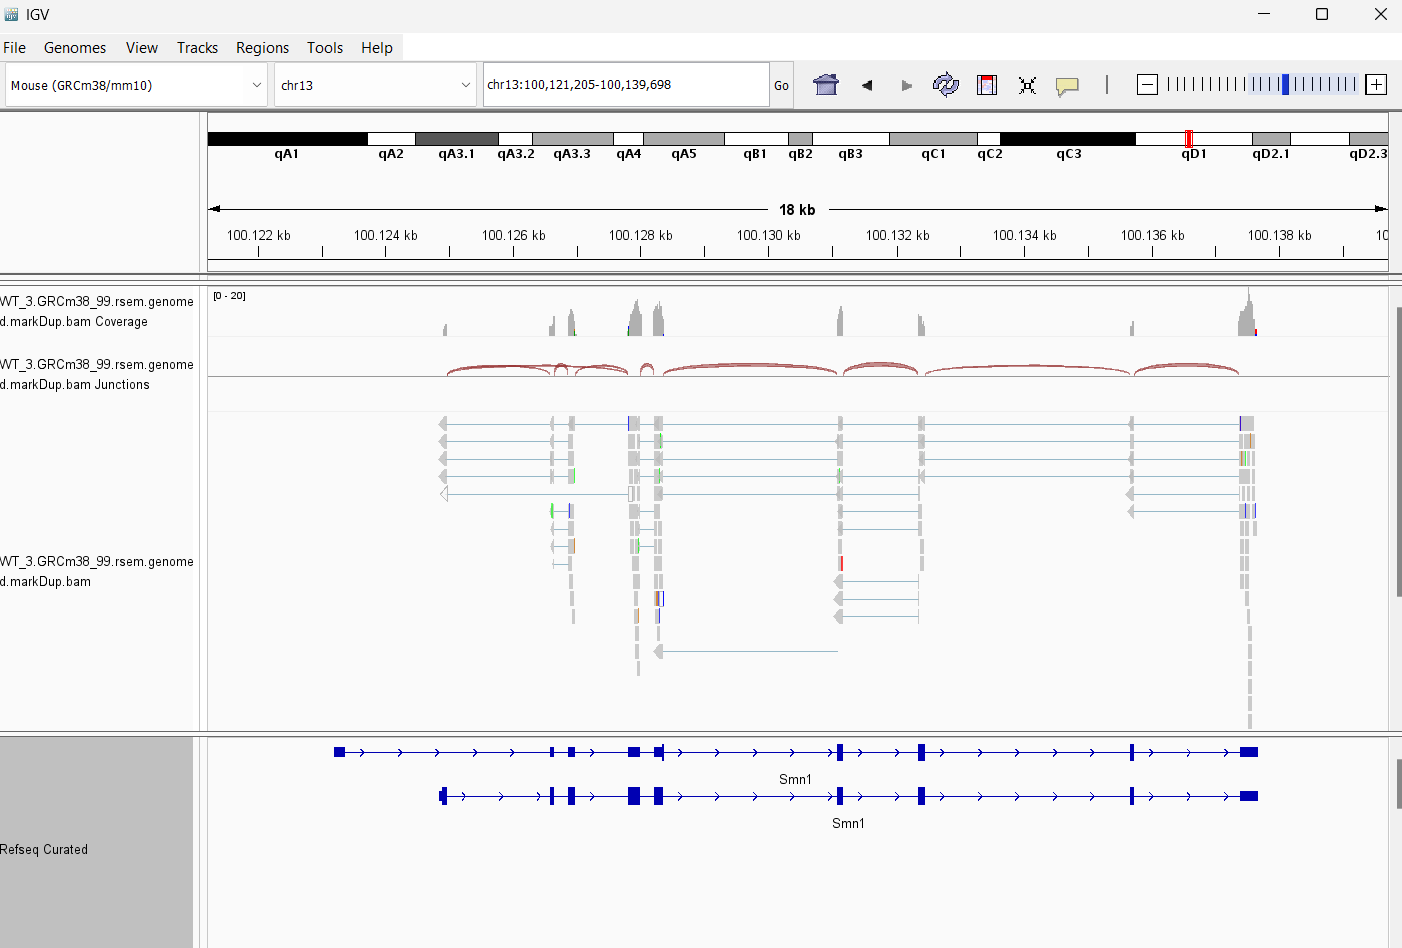
\includegraphics[width = 0.7\textwidth]{figs/igv-1.png}
\end{figure}

\subsection{Redundancia de mapeo}
Pueden darse redundancias de mapeo, ya que la secuencia del genoma es larga y contiene muchas secuencias repetitivas. Por ello, hay que mirar la calidad de mapeado, ya que una lectura puede mapear en un sitio con 1 mismatch y en otra región con 2. Para reducir la ambigüedad en el mapeado (hay genes pareados, isoformas), se puede utilizar pair-end o secuenciación de reads más largas. 

En NGS, se pueden detectar regiones por enriquecimiento viendo, en base a la cobertura del experimento, las regiones donde hay señal y que indicarán genes o factores de transcripción. El proceso es crosslinking, sonicación, inmunoprecipitación y secuenciación. El resultado de este tipo de experimento es un archivo tipo BED o WIG en el que se obtiene la posición donde se encuentra la señal.

En el conteo por ocurrencias, se cuentan cuántas reads caen en las distintas regiones. Para ello se requiere el GTF que asocia los disitntos exones con los tránscritos o isoformas.

En Galaxy, se puede utilizar un solo programa para alinear las lecturas a la referencia y la cuantificación. Al final, no importa si una read pertenece a una isoforma o a otra si queremos abstraer la cuantificación de una proteína, es decir, obtener la cuantificación absoluta. Para la expresión diferencial, se necesita más cobertura y los métodos son un poco diferentes para poder diferenciar las isoformas. Los tránscritos tienen una estructura de dependencia muy complicada, por lo que la expresión diferencial se suele hacer a nivel de gen.

\subsection{Cálculo de expresión}
Una vez con las lecturas mapeando a un gen, si queremos tener una medida robusta de la expresión, hay que tener en cuenta la longitud del gen y el tamaño de la librería. Una librería con una secuenciación mayor, la expresión va a parecer mayor que en una secuenciación con un tamaño menor de librería. Además, un tránscrito más corto va a tener menos reads que caigan en él por mera probabilidad, por lo que hay que normalizar por el tamaño del gen. Para ello, primero se obtienen los counts (la cobertura) y se utilizan los RPKMs:
$$RPKM: 10^9 \cdot \frac{\text{Reads mapped to the transcript}}{\text{Total reads} \cdot \text{Transcript length}}$$
Esta fórmula se modificó a la siguiente para normalizar todo a la vez:
$$TPM = 10^6 \cdot \frac{\text{reads mapped to transcript / transcript length}}{\sum \text{reads mapped to transcript/transcript length}}$$

Para las reads que mapean a varias isoformas o a varios genes del genoma, se utilizan los programas RSEM, Salmon o Sailfish. Estos métodos son procesos iterativos. Se aprovechan de la información de todos los reads para mejorar la probabilidad de qué read pertenece a qué sitio. Teniendo tres isoformas que coinciden en el primer exón, se ven las reads que caen en las partes distintas de los tránscritos para inferir las reads de la parte común de los tránscritos. La probabilidad se va cambiando y ajustando según cambian las probabilidades. Estos métodos probabilísticos hacen una estimación de los counts. Estos algoritmos cuantifican la expresión por isoforma, ya que están hechos para lidiar con el multimapping. La columna IsoPct indica el porcentaje de expresión de esa isoforma sobre toda la expresión del gen completo. Cuando se ve un proceso de splicing alternativo, la isoforma mayoritaria es la primera, y en otra condición puede darse que todas las isoformas estén igual de expresadas o que se convierta en la menos expresada.

El gen SMN1 de ratón es esencial, no puede haber ninguna mutación al ser inviable. De hecho, en humanos, una mutación en este gen causa SMA (spinal muscular atrophy). Esto se debe a que tenemos otro gen, SMN2, que solo se diferencia del 1 en una base y puede ayudar a compensar. Aunque las reads sean prácticamente idénticas, RSEM es capaz de asignarlas a una forma u otra.

\begin{figure}[h]
\centering
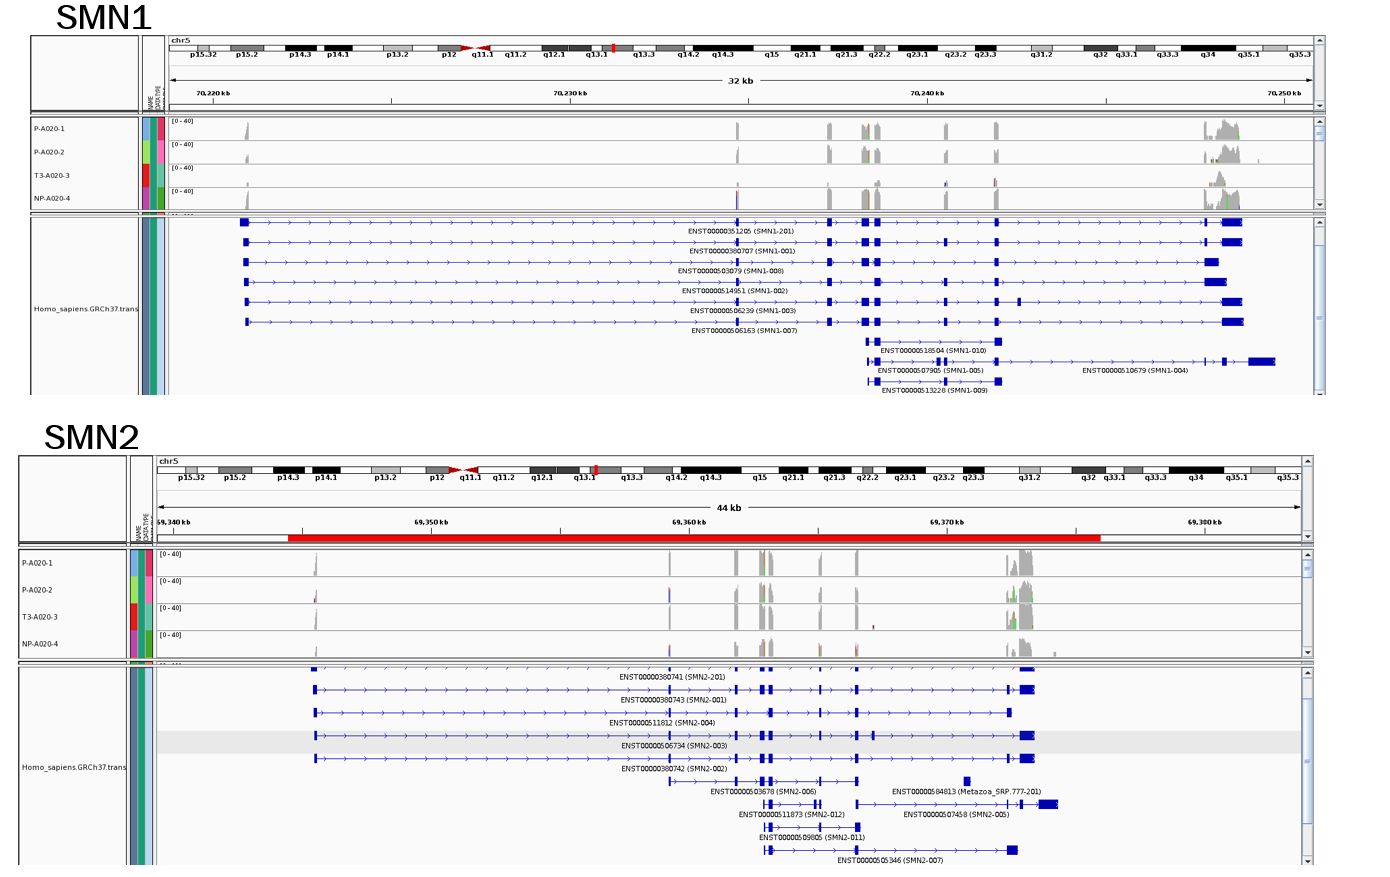
\includegraphics[width = 0.7\textwidth]{figs/smn12.png}
\end{figure}

\subsection{Galaxy}
Volviendo a la práctica, nos vamos a Ensembl y BioMart. Seleccionamos el genoma de ratón, seleccionamos como atributos solo Gene stable ID y transcript stable ID (quitamos los version) y exportamos los resultados como tsv. En Galaxy subimos ese fichero (Gene2Transcript) y utilizamos la herramienta "Sort Column Order by heading" para poner la columna 2 como identificador. 

El siguiente paso es construir la referencia del tránscrito (el fasta del transcriptoma) a partir del GTF que habíamos subido previamente con la herramienta gffread. Debería coger automática el fichero gtf, y en caso contrario lo seleccionamos manualmente. En el apartado de Reference Genome, debemos poner "From your history" para poder indicar el fasta. Además, en "select fasta outputs", seleccionamos la opción de "fasta file with spliced exons for each GFF transcript". También hay que activar "full GFF attribute preservation", y en Feature File Output poner GTF.

%12/02 - Fátima
A continuación utilizamos salmon\_qual utilizando el fichero exons.fa que se acaba de generar.
Los alineadores/mapeadores alinean los reads base a base y cuantifican por exón, tránscrito y gen el número de reads que caen en cada una de esas regiones. Por ello, debe recibir la referencia exons.fa creado a partir del GTF y del Fasta. También recibe la tabla que mapea los tránscritos a los genes (la que hemos construido con el sort column) para conseguir la cuantificación por gen. Aunque nosotros hayamos utilizado salmon, existen otros algoritmos como sailfish y RSEM. En RNA-Seq no quitamos los duplicados al poder significar una mayor expresión. Además, los tres métodos permiten el multimapping para poder ver si las reads van a una u otra isoforma mediante métodos estadísticos de expectation-maximization. 

El resultado contiene el gen (no tránscrito, eso sería otro análisis), la longitud del gen, la longitud efectiva (la que se puede mapear), los TPMs y el número de reads. Esto último es el dato crudo de cuántas reads del experimento caen en ese gen, mientras que los TPMs son los datos normalizados. Para el análisis de expresión diferencial, vamos a utilizar las reads crudas. 

\section{Análisis de expresión diferencial}
\subsection{Galaxy}
Para el análisis de la expresión diferencial, necesitamos una tabla con el ID del gen y las columnas con los reads. Esto lo vamos a hacer dentro de Galaxy con la función cut con el output de salmon y escogiendo las columnas 1 y 5. El siguiente paso es utilizar columnjoin sobre este resultado, siendo la columna 1 el identificador y con 1 línea de encabezado en cada fichero de input.

Con los counts normalizados por el tamaño de gen y de librería, si hiciéramos un plot de expresión sobre lgFC, habría más variabilidad a baja expresión. Limma-voom y trend permite estabilizar la varianza para poder realizar posteriormente el test estadístico. El ejemplo en el que estamos trabajando es bastante sencillo, pero para cuando nos veamos en situaciones más complejas (varias condiciones, medidas repeticas, etc) hay un tutorial de limma escrito por su autor, Gordon Smyth. voom permite meter información sobre la calidad de las réplicas, pero en este caso no vamos a usarlo. Seleccionamos single count matrix. El factor es la variable que determina las condiciones. Por ello, nosotros vamos a añadir un factor llamado genotype y damos para cada muestra el grupo al que pertenece. Esta información está en los metadatos; las primeras tres muestras son WT y las otras tres KO, por lo que debemos proporcionar lo siguiente: WT, WT, WT, KO, KO, KO. 

En Ensembl BioMart, seleccionamos Ensembl Genes y Mouse genes. En Attributes, debemos marcar Gene stable ID y Gene Name y obtener los resultados únicos. Con los resultados descargados, en Galaxy permitimos Gene Annotations y subimos este fichero. Este paso es opcional, es simplemente para que podamos ver mejor los genes. En contrast, debemos poner KO-WT.

A la hora de hacer el análisis de expresión diferencial, cuantas más hipótesis (genes) testemos, más habrá que corregir el p-valor. Por ello, genes no expresados, no aportan información y aumentan el error de tipo 1. Por ello, se pueden quitar los filtrados. En este caso, no queremos quitar aquellos genes que entre las dos condiciones esté downregulado (y en KO no tenga expresión, por ejemplo), pero si un gen no está expresado en más de 4 muestras (de 3 que tenemos por cada condición), sí podemos quitarlos, por lo que sí permitimos el filtrado de genes poco expresados. El filtrado se hace en base de las CPM, poniendo que haya al menos 1 count por million en al menos 3 muestras. Dentro de opciones de salida, seleccionamos todos los posibles plots. 
%esto es lo que pedirá en el ejercicio para que los interpretemos
Del output, siempre hay que usar el p-valor ajustado. 

Por detrás, se ha ejecutado un script de R, que lo veremos más en detalle a continuación. Utilizamos el script \texttt{limma\_example\_rma.r} localizado en la carpeta de prácticas. 

De Galaxy, nos descargamos la tabla resultante (localizada en carpeta de prácticas): Galaxy64-[limma-voom\_KO-WT].tabular. 
Ahora tenemos una colección de genes diferencialmente expresados y tenemos dos opciones: ir mirando uno a uno los genes (por ejemplo, Nlr tiene un p-valor ajustado de $10^{-12}$ y un logFC de -8, es un gen utilizado para el Knock-Out y verificamos que ha funcionado bien. A partir de ahora, buscaríamos rutas de genes que se verían afectados con el KO de este gen. 

Hay dos tipos de análisis funcional: 
\begin{itemize}
\item \textbf{ORA (overrepresentation analysis):} Tenemos 6407 genes diferencialmente expresados de 18387 (obtenidos mediante un filtro de p-valor ajustado < 0.5). Cada uno de los genes se puede clasificar en función del proceso biológico en el que está involucrado (biological process; BP), la función molecular (molecular function; MF) o el compartimento celular (cellular compartment; CC). Para un gen, podemos buscar esto en Gene Ontology Overview. Dentro de cada categoría, hay muchas clases que permiten clasificar los genes de forma cada vez más específica, y un gen puede estar en varias clases. Podemos escoger el número de procesos y la profundidad que deseamos. Asignamos así cada gen a un proceso, y contamos para cada proceso cuántos DEGs hay. Este número se compara con los valores de Whole genome. Aquellas proporciones muy enriquecidas son las que se marcan como cambio significativo. Así, se puede decir que el experimento afecta sobre todo al proceso x (por ejemplo, regulación génica). En caso de no obtener ningún DEG, se podrían utilizar filtros más laxos, o utilizar GSEA. 
\item \textbf{GSEA (gene set enrichment analysis):} para este método, se cogen la lista de todos los genes y se ordenan de menor a mayor en función de su logFC (aunque se puede elegir en función de qué hacer la ordenación). Seguimos teniendo la lista con los procesos a los que pertenecen los genes. Por ello, podemos ver dónde caen los genes de cada proceso. Si para un proceso todos los genes se encuentran cerca, esto se puede reportar (tienen una magnitud de cambio similar; el experimento perturba ese proceso). 
\end{itemize}
 
En el NIH está la herramienta \href{https://davidbioinformatics.nih.gov/}{DAVID} que permite subir una lista o un background (pestaña functional annotation). En el caso de los arrays, no se miran todos los genes, por lo que no tiene sentido comparar en el ORA con whole genome, si no que se utiliza otro background (por ejemplo, solo el cromosoma 1, lo que se utilice como total). En nuestro caso copiamos los primeros 150 gene ID, pero también se podría subir en forma de fichero. Se selecciona que los identificadores sean de genes de Ensembl y que se trata de una lista, no background. Hay 14 genes que no se pueden detectar con esta herramienta, pero es algo asumible. Aparece una pestaña de Gene Ontology que especifica los distintos niveles de las tres partes (BP, MF y CC). Por ejemplo, para BP, hay 5 niveles, cada uno a un mayor nivel. En direct, se mezclan los distintos niveles para obtener una clasificación que sea detallada, pero sin ser exhaustiva. Como se están testando muchos genes, hay que volver a hacer el ajuste del p-valor, que en este caso aparece en una columna con la corrección de Benjamini. Esto sería el equivalente al ORA.
%Importante describir bien esta parte.

%14/02 - Carlos Torroja
\chapter{ChIP-Seq}
\section{Procedimiento experimental}
ChIP-Seq (Chromatin Immunoprecipitation Sequencing) es una técnica diseñada para identificar las regiones del ADN donde se unen los factores de transcripción. Utiliza secuenciación de nueva generación (NGS) de lecturas cortas (short reads) y se basa en la inmunoprecipitación de factores de transcripción. Si no se dispone de un anticuerpo específico para el factor de transcripción de interés, la técnica no puede llevarse a cabo.

El procedimiento experimental es el siguiente:
\begin{enumerate}
\item \textbf{Fijación y fragmentación del ADN:} Se fijan las células de un tejido con un agente químico para mantener el factor de transcripción unido al ADN. Se extrae el ADN junto con las proteínas unidas y se fragmenta mediante sonicación, obteniendo fragmentos de aproximadamente 200 pares de bases, ideal para la secuenciación con tecnología Illumina. Este tamaño permite además acotar la región donde buscar posteriormente los enriquecimientos.
\item \textbf{Inmunoprecipitación:} Se introduce un anticuerpo específico para el factor de transcripción en la solución de fragmentos de ADN.
Como control, se puede preparar una muestra sin anticuerpo para evaluar la distribución del coverage del genoma.
Los fragmentos de ADN unidos al factor de transcripción se capturan utilizando una columna con bolitas que se unen a la región constante del anticuerpo.
\item \textbf{Preparación de la librería y secuenciación:} Se deshace la fijación para eliminar las proteínas y se prepara la librería de ADN para secuenciar.
Se realiza la secuenciación, idealmente obteniendo entre 20 y 40 millones de lecturas (reads).
\end{enumerate}

\section{Análisis de Datos}
\paragraph{Alineamiento de lecturas}
Las lecturas se alinean al genoma de referencia. En general, se utiliza secuenciación single-end, donde las lecturas no están pareadas.
Se observa un patrón donde las lecturas se alinean en la región 5' en un sentido y en la región 3' en sentido inverso, lo que indica la señal de enriquecimiento.

\paragraph{Identificación de regiones enriquecidas}
Se utilizan herramientas como MACS (Model-based Analysis of ChIP-Seq) para identificar regiones enriquecidas.
MACS modela una distribución nula, fragmenta el genoma en bins y calcula el número de lecturas en cada bin.
La herramienta desplaza y junta los picos de las distribuciones (una por cada sentido) para aumentar la señal y evaluar las regiones enriquecidas en comparación con el control.

\paragraph{Análisis de motivos de unión}
Se identifican las secuencias de ADN donde se une el factor de transcripción y los genes asociados.
Se utilizan herramientas para buscar motivos enriquecidos de 10-15 nucleótidos mediante el algoritmo de expectation-maximization.
Esto permite estimar la secuencia consenso de unión y predecir otros sitios potenciales en el genoma mediante el logo generado.

\section{Aplicación práctica: Pipeline de análisis con Galaxy}
\subsection{Obtención de datos}
Vamos a construir una pipeline para analizar datos de ChIP-Seq del artículo \href{https://www.sciencedirect.com/science/article/pii/S2211124713001368?via\%3Dihub}{"Analysis of the DNA-binding profile and function of tale homeoproteins reveals their specialization and specific interactions with hox genes/proteins"}. Este estudio evalúa los sitios de unión de tres factores de transcripción: Prep1, Meis1 y Pbx1, relacionados con los genes Hox del desarrollo embrionario.

En este estudio se realizaron tres ChIP-Seqs con tres anticuerpos, uno para cada factor. Meis1 salió muy ruidoso, Prep1 tenía unos picos muy marcados, y Pbx1 mostró algo intermedio. Los picos de Meis tenían dos distribuciones, y donde estaba Prep, Meis también tenía un pico marcado. 

Para esta pipeline utilizamos el \href{https://usegalaxy.org/}{servidor americano de Galaxy}. Ahí podemos buscar en historias públicas la historia "Pbx1 ChIPSeq Raw Data" del usuario "cartof", que es Carlos Torroja (el profesor). Los datos del artículo están disponibles en GEO, y podemos acceder desde la sección de "Additional Information" de PubMed. Desde ahí podemos navegar a SRA Run Selector, donde aparecen todas las muestras del artículo. Hay dos tipos de assays, RNA-Seq y ChIP-Seq, por lo que seleccionamos solo aquellas pertenecientes a ChIP-Seq. Hay un botón de "Computing Galaxy" que importa los datos directamente al servidor americano; para utilizar el servidor europeo, habría que descargar las tablas de metadatos e importarlas manualmente como se hizo en la pipeline de RNA-Seq.

\subsection{Preprocesamiento de datos}
Los datos ya están subidos a Galaxy, pero hay que preprocesar el contenido. Las anotaciones de los campos son libres, no hay estándar, por lo que la pipeline se debe adaptar a los datos concretos. 
En este caso, solo nos queremos quedar con tres columnas: la columna 1 run con los identificadores SRR, la columna 17 con el nombre de la librería y la columna 32 con el nombre del anticuerpo utilizado. Para esto, utilizamos la herramienta \texttt{cut columns}. Tras ver el resultado, vemos que algunas celdas contienen "signos prohibidos" en bioinformática, como espacios o paréntesis. Por ello, el siguiente paso es utilizar \texttt{column regex find and replace}. Esto se debe ejecutar dos veces:
\begin{enumerate}
\item \textbf{Columna 2}: debemos realizar dos comprobaciones. Primero, se sustituye .*WT\symbol{92}s([\symbol{92}w\symbol{92}s]+) por \symbol{92}1. El segundo check debe buscar \symbol{92}s y reemplazar por \_.
\item \textbf{Columna 3}: buscamos [\symbol{92}/\symbol{92}s].+ y lo queremos reemplazar por nada, por lo que se deja el campo en blanco.
\end{enumerate}

\subsection{Descarga y extracción de lecturas}
Hasta ahora, hemos realizado los pasos anteriores directamente en la historia. Los siguientes pasos los vamos a crear como parte de un flujo de trabajo, creando un nuevo workflow desde la pestaña con ese mismo nombre. Los flujos de trabajo se construyen con casillas que representan distintas entradas o herramientas, pudiendo ordenar todo.

Primero incluimos una casilla de "input database" que llamamos SRA Table con descripción "Sample table with SRR column and sample name column" y formato tabular. A continuación añadimos la herramienta "cut" con nombre "Extract SRR Column", desactivando los parámetros de la herramienta. De esta forma, a la hora de lanzar el flujo de trabajo, se pide al usuario la introducción de las columnas que se desean mantener. La alternativa sería, en lugar de desactivar el parámetro, generar una entrada que se utilice en la herramienta. Esto se consigue pulsando el icono de las dos flechas, permitiendo así enlazar una casilla de "input" con la herramienta.

La primera fila del fichero contiene la cabecera de las columnas, y no queremos que forme parte del análisis bioinformático. Para ello, incluimos una casilla con la herramienta "select last lines from a database (tail)". Entre los parámetros, debemos especificar "keep everything from this line on" y "2", de manera que siempre se vaya a eliminar la cabecera.

El flujo de trabajo contiene por ahora solo pasos intermedios. Para evitar su aparición en la historia cuando se lance el flujo, generando ruido visual, se pueden ocultar pulsando sobre el símbolo del ojo. Ahora ya podemos incluir la herramienta "Faster Download and Extract Reads in FastQ format". Por defecto, no permite introducirle una entrada, primero hay que seleccionar la opción de "list of SRA accession, one per line". La salida de esta herramienta se divide en cuatro. Para una secuenciación single-end, debemos trabajar con la salida "output\_collection", mientras que para una secuenciación pair-end, "list\_paired".

\begin{figure}[h]
\centering
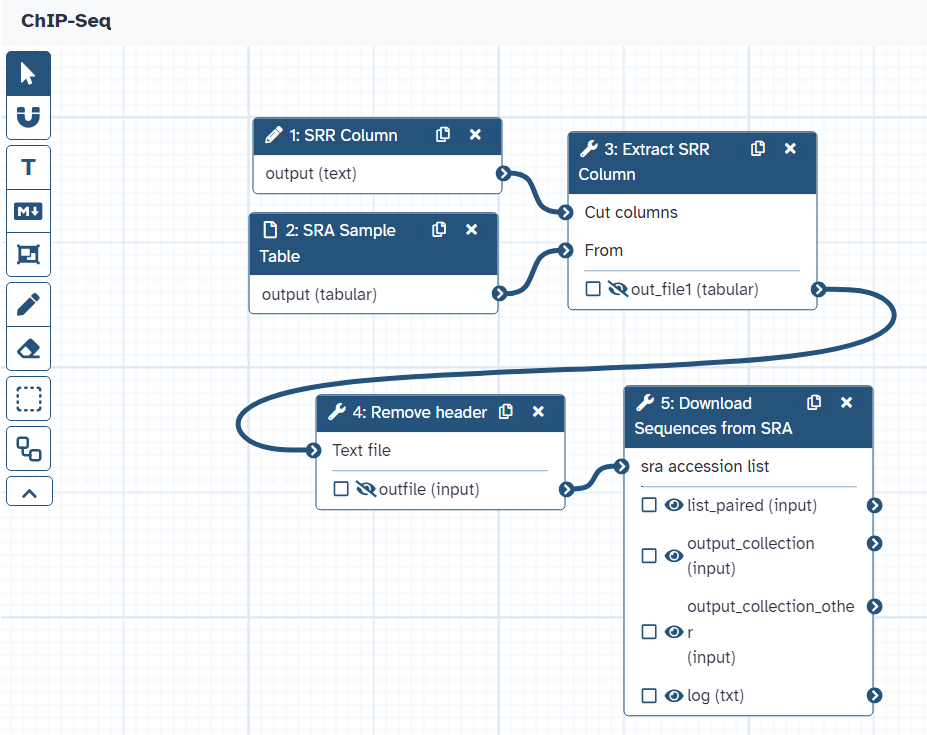
\includegraphics[width = 0.6\textwidth]{figs/chipseq-workflow-start.png}
\end{figure}

\subsection{Análisis posterior}
Los siguientes pasos del análisis serían realizar un control de calidad con FastQC y utilizar una herramienta de trimmeado (como Trim-Galore) para eliminar los adaptadores de la secuencia, aumentando así la capacidad de alinear. A continuación se podría pasar al alineado para saber la parte del genoma de donde provienen las lecturas mediante herramientas como BWA. En el FastQC se podría ver el tamaño de las regiones, que en este caso son de unos 35 nucleótidos, por lo que se puede utilizar la herramienta BWA estándar al no necesitar incluir gaps u otros eventos complejos más propios de secuencias más largas.

El resultado es un fichero BAM que se utiliza a continuación para realizar un control de calidad con la herramienta \texttt{plotFingerprint}. Del genoma se obtienen fragmentos pequeños que se utilizan para contar las lecturas que caen en cada fragmento. Esto se calcula para todas las muestras, y posteriormente se genera un gráfico que muestre la información: fragmentos por counts y un gráfico cumulativo.

En un análisis de ChIP-Seq, no hay un genoma de referencia, por lo que es necesario incluir un paso de detección de los picos de lectura. Esta detección se realiza en base a un patrón o en base al enriquecimiento. Esto se realiza con la herramienta MACS, la cual se encarga de la detección, del conteo y del análisis estadístico. Se identifican las regiones enriquecidas a través de la distribución de las lecturas. Se deben encontrar dos distribuciones, una para cada sentido de lectura. MACS puede detectar una distribución y emplearla para buscar una distribución opuesta en el rango de la sonicación (es decir, unos 200 pares de bases que se especifican como parámetro). A continuación junta ambas distribuciones en un pico central para aumentar la detección. 
%Para definir un tránscrito, debe estar enriquecido y cumplir con un patrón. En el caso de los picos, la detección es simplemente "enrichment-based". El transcriptoma debe ser compatible con las características que queremos detectar (miRNA, mRNA, sitio de unión a factor de transcripción). 
El siguiente paso es la búsqueda en distintos tamaños de fragmento, quedándose con el que mejor se adapte y simulando la distribución nula con los datos. Además, se pueden modificar el tamaño efectivo del genoma de referencia e incluir en las salidas adicionales la de "peak summits". 

El resultado es un fichero bed que se debe ordenar según el score. Este fichero se emplea para la búsqueda de los motivos de unión del factor de transcripción. En el fichero bed se incluyen las posiciones del nucleótido donde empieza y donde termina, por lo que debemos aumentar el número en 50 nucleótidos en ambas direcciones (restar 50 a la posición de inicio y sumar 50 a la de fin). De la colección de regiones, se pueden filtrar las 500 entradas más altas y utilizar la herramienta "Extract Genomic DNA" para obtener la secuencia de esas posiciones. Con esto se puede utilizar la herramienta "MEME", obteniendo así los logos. Pulsando la flecha en Submit/Download, podemos buscar ese logo en la base de datos para encontrar otras secuencias iguales recogidas en ella.
%19/02 - José Manuel Rodríguez
\part{Proteómica y Metabolómica}
\chapter{Introducción a la proteómica y la espectrometría de masas}
\section{Introducción}
El \textbf{proteoma} se define como el conjunto completo de proteínas que se expresan, o pueden expresarse, a partir del genoma de una célula, tejido u organismo en un momento y condición específicos. La \textbf{proteómica}, por su parte, es la disciplina científica que estudia el proteoma mediante técnicas sistemáticas para identificar, cuantificar y caracterizar proteínas. Entre las herramientas más utilizadas en proteómica se encuentran la electroforesis, la espectrometría de masas (MS), la resonancia magnética nuclear (RMN), la microscopía óptica y electrónica, y la espectroscopía infrarroja por transformada de Fourier, entre otras.

\subsection{Análisis de proteínas por electroforesis}
La electroforesis es una técnica clásica de separación de proteínas basada en su carga eléctrica y masa molecular. En este método, las proteínas se separan en un gel según su punto isoeléctrico (pI), que es el pH al cual una proteína tiene una carga neta cero. Posteriormente, se realiza una segunda separación en función del peso molecular. Esta técnica ha sido fundamental en la proteómica "clásica" y sigue utilizándose para la validación de biomarcadores.

Tras la separación, el gel puede cortarse para aislar las proteínas de interés, las cuales se someten a una digestión con proteasas (como la tripsina) para generar péptidos. Estos péptidos pueden analizarse posteriormente mediante espectrometría de masas.

Sin embargo, la electroforesis presenta limitaciones: no es automática, tiene baja reproducibilidad y no es adecuada para proteínas grandes o hidrofóbicas. Además, suele ser efectiva solo para proteínas altamente abundantes. Estas limitaciones llevaron al desarrollo de la proteómica "Bottom-Up", que supera muchos de estos problemas.

\section{Proteómica "Bottom-Up"}
La proteómica "Bottom-Up" es un enfoque moderno que se basa en la digestión de proteínas en péptidos, seguida de su análisis mediante cromatografía líquida acoplada a espectrometría de masas (LC-MS). Este método es más sensible, reproducible y adecuado para el análisis de proteínas de baja abundancia.

\subsection{Digestión tríptica}
El primer paso en la proteómica "Bottom-Up" es la digestión de las proteínas. Las proteínas, en su estado nativo, están plegadas y pueden contener enlaces disulfuro que estabilizan su estructura. Para facilitar su análisis, las proteínas se desnaturalizan utilizando agentes como el dodecilsulfato sódico (SDS), que rompe los enlaces disulfuro y despliega las proteínas. Una vez desnaturalizadas, se someten a una digestión con tripsina, una enzima que corta específicamente después de los residuos de lisina (K) y arginina (R), generando péptidos de tamaño adecuado para su análisis por espectrometría de masas.

\subsection{Fraccionamiento para reducción de complejidad}
Tras la digestión, los péptidos resultantes pueden fraccionarse para reducir la complejidad de la muestra. Esto es especialmente útil en muestras que contienen múltiples proteínas o especies. El fraccionamiento puede realizarse mediante técnicas como la cromatografía de fase reversa, donde los péptidos se separan según su hidrofobicidad. Este paso permite una introducción más controlada y ordenada de los péptidos en el espectrómetro de masas.

\subsection{Cromatografía líquida y espectrometría de masas}
Los péptidos, fraccionados o no, se introducen en un sistema de cromatografía líquida (LC). Aquí, los péptidos se separan en función de su interacción con la fase estacionaria, lo que permite su elución en tiempos específicos. A medida que los péptidos salen de la columna cromatográfica, se ionizan mediante técnicas como la ionización por electrospray (ESI), formando gotitas cargadas que contienen los péptidos ionizados. A medida que el solvente se evapora, los péptidos ionizados entran en el espectrómetro de masas.

\subsubsection{Componentes del espectrómetro de masas}
Un espectrómetro de masas consta de los siguientes componentes principales:
\begin{itemize}
\item \textbf{Sistema de introducción de muestras}: Introduce los péptidos ionizados en el espectrómetro.
\item \textbf{Cámara de ionización}: Aquí, los péptidos se ionizan. Una de las técnicas más comunes es la ionización por electrospray (ESI).
\item \textbf{Analizador}: Determina la relación masa-carga (m/z) de los iones. Existen diferentes tipos de analizadores, como los de cuadrupolo, tiempo de vuelo (TOF) y trampa de iones.
\item \textbf{Detector}: Registra la masa y la intensidad de los iones detectados.
\end{itemize}

\begin{figure}[h]
\centering
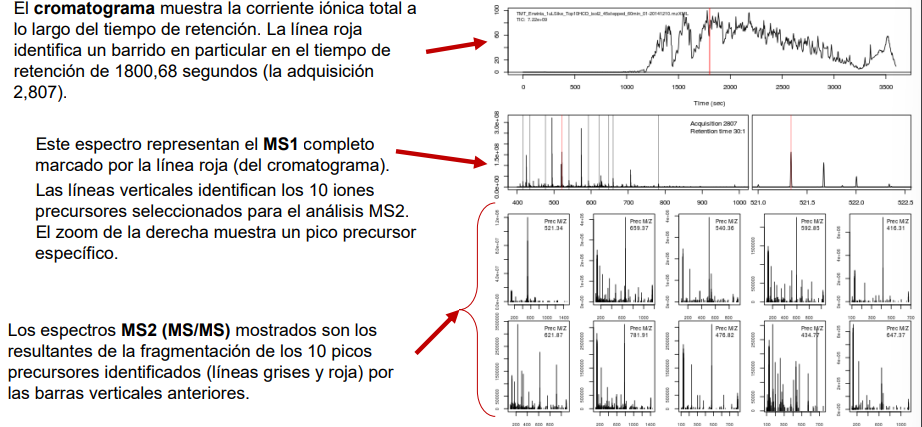
\includegraphics[width = \textwidth]{figs/espectro-analisis.png}
\caption{La figura superior indica el cromatograma obtenido. Primero hay un tiempo de retención con la intensidad encontrada de toda la carga iónica recibidas. A partir de un tiempo de retención señalado con la línea roja, empieza el tiempo de adquisición. El MS1 (panel central) es la ampliación de la línea roja del cromatograma. Cada línea vertical indica la masa detectada con sus intensidades. La parte derecha es un zoom de la línea roja. El MS1 se genera por cada péptido encontrado. Para este ejemplo, se cogen los iones marcados en gris y rojo y se fragmentan. Se saca la masa, carga e intensidad por cada uno de los iones en el segundo analizador. }
\end{figure}

La siguiente imagen muestra una representación de un LC-MS. A partir de un determinado tiempo de retención, hay una serie de masas cargas de los péptidos con una intensidad asociada a cada uno. Para diferentes tiempos de retención hay diferentes picos del espectrómetro.

\begin{figure}[h]
\centering
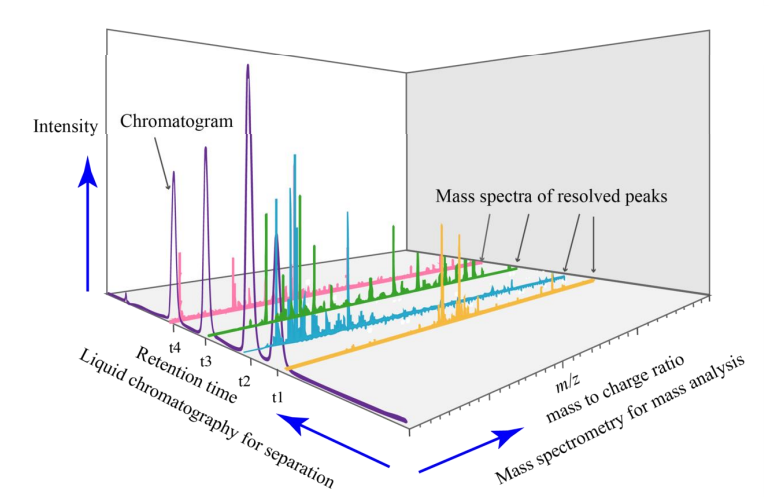
\includegraphics[width = \textwidth]{figs/lc-ms.png}
\end{figure}

Se tienden a coger los picos con mayor intensidad, ya que el resto son ruido del espectrómetro. Se sabe que a la hora de tener los péptidos, hay unos iones que van del extremo N-terminal al C-terminal y otros que van en sentido contrario. Estos iones van calculando la masa acumulativa. De esta forma se pueden saber los aminoácidos que componen el espectro.

\begin{figure}[h]
\centering
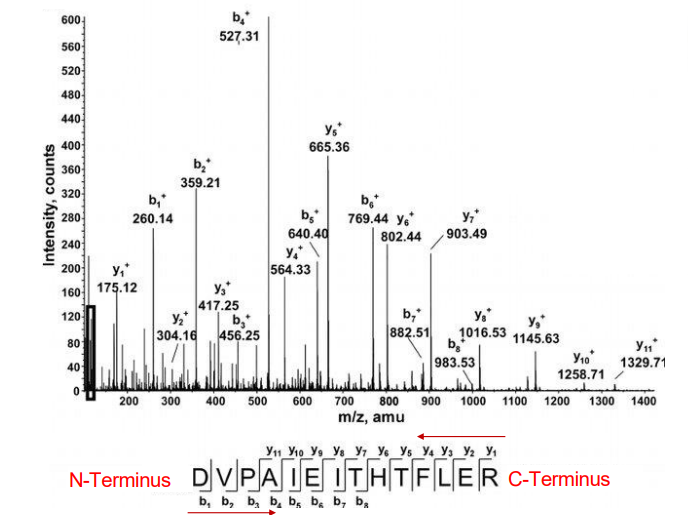
\includegraphics[width = 0.6\textwidth]{figs/fragmentacion-msms.png}
\end{figure}

\subsection{Adquisición de datos}
La adquisición de datos en espectrometría de masas puede realizarse de dos formas principales:
\begin{itemize}
\item \textbf{Adquisición dependiente de datos (DDA)}: En este modo, los iones más abundantes detectados en el espectro MS1 se seleccionan para su fragmentación, generando espectros MS2. Este proceso se repite secuencialmente para múltiples iones.
\item \textbf{Adquisición independiente de datos (DIA)}: En este modo, se fragmentan regiones específicas del espectro MS1, independientemente de la intensidad de los iones. Esto permite la detección de iones de baja abundancia, aunque puede resultar en espectros MS2 más complejos debido a la co-fragmentación de múltiples péptidos.
\end{itemize}

\begin{figure}[h]
\centering
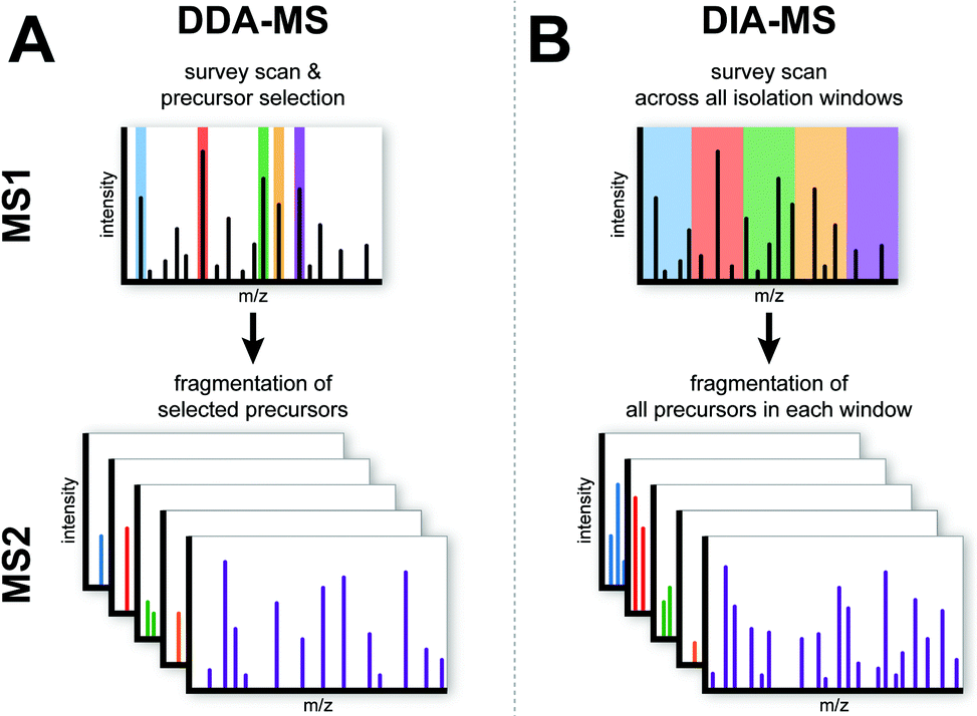
\includegraphics[width = 0.6\textwidth]{figs/data-adquisition.png}
\end{figure}

\subsection{Identificación de péptidos y proteínas}
La identificación de péptidos y proteínas se realiza comparando los espectros experimentales con bases de datos teóricas. Estas bases de datos contienen información sobre las masas y secuencias de péptidos generados in silico a partir de proteínas conocidas. Al comparar los espectros experimentales con los teóricos, se puede determinar la secuencia de aminoácidos de los péptidos y, por tanto, identificar las proteínas presentes en la muestra. Cada identificación se asocia con un score de confianza que indica la fiabilidad del resultado.

\subsection{Aplicaciones de la proteómica "Bottom-Up"}
La proteómica "Bottom-Up" tiene dos enfoques principales:
\begin{itemize}
\item \textbf{Proteómica de descubrimiento (Discovery Proteomics)}: Se utiliza para analizar proteomas completos, identificando y cuantificando proteínas de abundancia moderada a alta. Un posible ejemplo es la búsqueda de posibles biomarcadores.
\item \textbf{Proteómica dirigida (Targeted Proteomics)}: Se centra en la cuantificación de proteínas específicas, incluso en bajas abundancias. Una técnica común en este enfoque es el monitoreo de reacciones seleccionadas/múltiples (SRM/MRM), que utiliza tres analizadores de cuadrupolo para seleccionar y cuantificar péptidos específicos. Un ejemplo de aplicación es la validación de biomarcadores.
\end{itemize}

\subsubsection{Cuantificación y estándares internos}
En la cuantificación de proteínas, es crucial utilizar estándares internos para corregir variaciones en la ionización y la eficiencia de la cromatografía. Estos estándares son péptidos sintéticos con propiedades similares a los péptidos de interés, pero marcados con isótopos estables. Al comparar las áreas bajo la curva de los péptidos de interés con las de los estándares internos, se obtiene una cuantificación precisa y reproducible.

\begin{figure}[h]
\centering
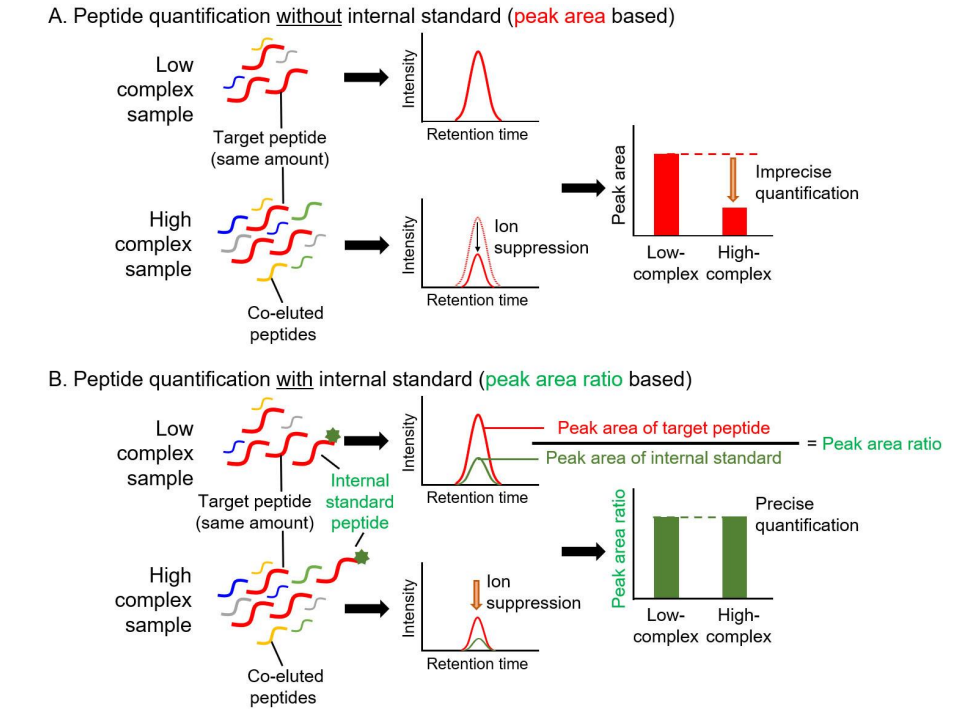
\includegraphics[width = 0.8\textwidth]{figs/internal-standard.png}
\end{figure}

%Cuando la muestra es compleja, los péptidos pueden competir causando colución. La intensidad va a disminuir al haber menos iones que se cuantificarán. La cuantificación de una muestra compleja será por tanto menor que el mismo péptido en una muestra poco compleja. Por esto, se establecen estándares internos: péptides con cualidades similares marcados. Se conoce la cantidad a priori del péptido asociado. Así, da igual si la complejidad es mucha o poca, ya que se establece la relación entre el péptido asociado y el péptido buscado. Lo que se calcula es el ratio del pico, es decir, el área del péptido buscado con el área del estándar interno. 

%21/02 - José Manuel Rodríguez
\section{Proteómica "Top-Down"}
En este caso, tenemos la proteína intacta y se calcula la masa con el espectrómetro. Se usan los mismos tipos de espectrómetros: cromatografía líquida y espectrómetro de masas. Químicamente, la muestra biológica no se desnaturaliza ni se digiere, si no que se sigue un protocolo de lisis para romper las membranas celulares. Dependiendo de las muestras y sus condiciones, las proteínas mantendrán su estructura o si están haciendo ligando, se mantendrán las relaciones. Si para esas condiciones de muestra hay alguna modificación post-traduccional, va a ser más fácil de identificar con esta técnica de Top-Down. 

Las proteínas intactas se pasan a un HPLC. Se realiza la ionización por electrospray y con el tiempo de retención y las intensidades, se obtiene la masa carga de toda la proteína (MS1). Posteriormente se fracciona en determinados puntos dentro de la proteína. Es más fácil obtener la estructura de la proteína. El MS2 permite ver la estructura de fragmentos de la proteína. 

En el caso del Bottom-Up, tenemos toda la proteína y se hace una digestión tríptica. Los péptidos se ionizan, y esos fragmentos ionizados son los que detectará el MS. En Top-Down, la proteína intacta se ioniza. Al fragmentar para el MS2, hay trozos y fragmentos de los iones con una conformación de la proteína más larga, siendo así más fácil ver la estructura completa. 

Comparando las dos técnicas en proteómica:
\begin{table}[h]
\centering
\begin{tabular}{p{4cm}|p{5cm}p{5cm}}
Aspecto & Top-Down & Bottom-Up \\ \hline
Tamaño de las proteínas & Adecuado para proteínas pequeñas y medianas & Adecuado para todo tamaño, especialmente proteínas grandes \\
Equipos & Instrumentos de alta resolución & Instrumentos más accesibles \\
Sensibilidad & Menor, difícil para proteínas en baja abundancia & Mayor sensibilidad \\
Complejidad computacional & Alta, espectros más difíciles de interpretar & Menor, espectros de péptidos más sencillos \\
Cobertura & Cobertura completa de la proteína & Cobertura parcial (depende de la digestión) \\
Manejo de mezclas complejas & Difícil para mezclas de muchas proteínas & Más fácil, adecuado para muestras complejas \\
Detección de PTMs & Precisa, localización directa en la proteína intacta & Puede perder algunas PTMs, pero identifica modificaciones en péptidos \\
Preparación de muestras & Más compleja, requiere proteínas intactas & Más sencilla, con digestión enzimática
\end{tabular}
\end{table}

\begin{figure}[h]
\centering
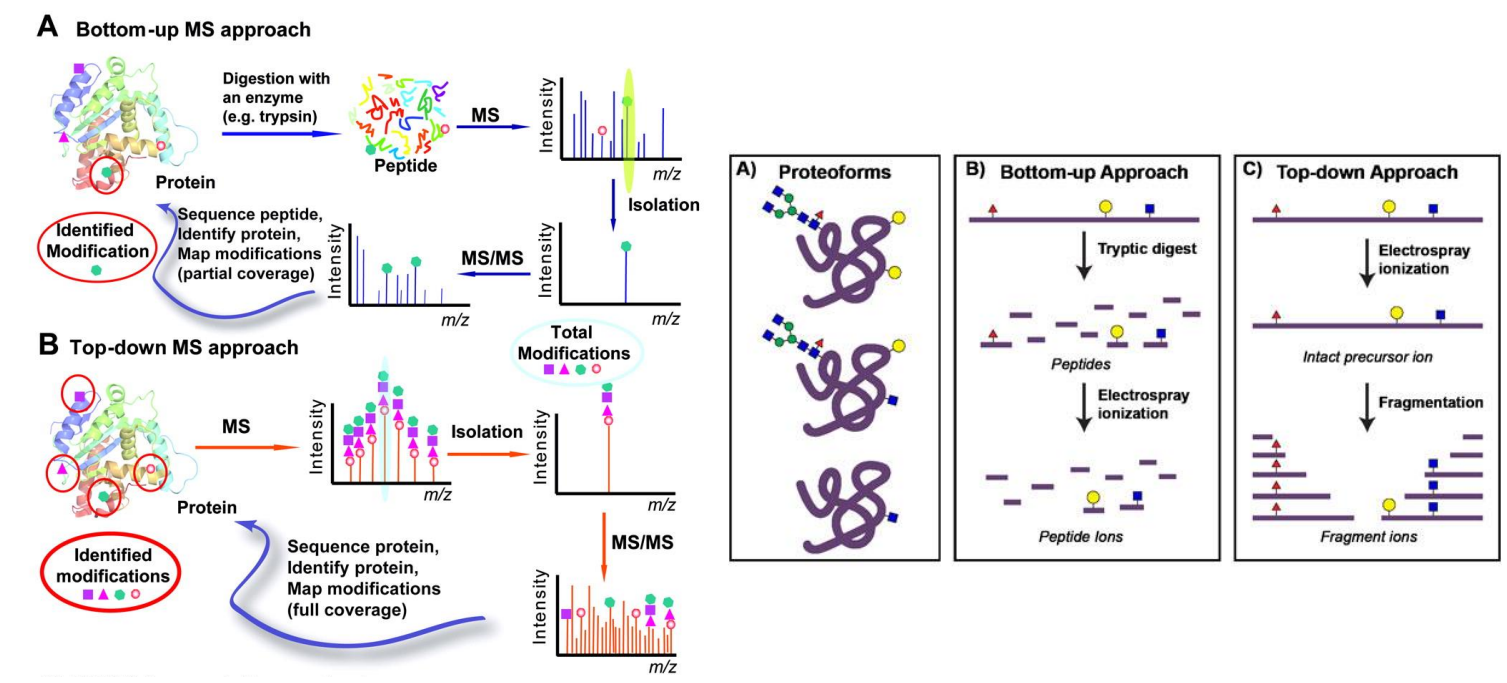
\includegraphics[width = 0.9\textwidth]{figs/topdown-vs-bottomup.png}
\end{figure}

\chapter{Identificación de péptidos mediante espectrometría de masas}
Las máquinas actuales generan millones de espectros MS/MS en muy poco tiempo. No se pueden interpretar manualmente, siendo necesario usar herramientas computacionales. 
Las estrategias más utilizadas para identificar péptidos mediante MS/MS son:
\begin{itemize}
\item \textbf{Secuenciación \textit{de novo}}: Consiste en obtener la secuencia del péptido directamente a partir del espectro.
Se usa en casos donde el genoma del organismo no está (o sólo parcialmente) secuenciado. La
secuencia se infiere directamente del espectro sin ayuda de una base de datos de referencia.
También se usa para identificar o caracterizar modificaciones postraduccionales.

\item \textbf{Búsqueda contra bases de datos}: Se identifica el péptido en la base de datos a partir del espectro MS/MS. Para ello se hace una "correlación" entre el espectro MS/MS obtenido experimentalmente y los espectros teóricos generados a partir de las secuencias de los péptidos en la base de datos.

Los motores de búsqueda se encargan de asignar a cada espectro obtenido experimentalmente un péptido, que es el mejor candidato de una lista de los posibles péptidos en la base de datos, de acuerdo a cierta \textbf{puntuación}, que mide el \textbf{grado de similitud entre el espectro empírico y el teórico}.
A cada una de estas \textbf{parejas péptido-espectro} se les denomina \textbf{PSM} (Peptide-Spectrum Match, Asignación Péptido-Espectro). 

Denominaremos \textbf{puntuaciones simples} a aquellos algoritmos que generan una puntuación para cada PSM que es independiente de la puntuación asignada al resto de PSMs en el mismo experimento.
Los algoritmos que asignan una puntuación a cada PSM considerando el comportamiento del resto de las PSM generan puntuaciones que denominaremos \textbf{complejas}.
\end{itemize}

\section{Algoritmos de identificación de péptidos - Puntuaciones simples}
Hay varios algoritmos para poder obtener esta puntuación:
\begin{itemize}
\item \textbf{Algoritmos empíricos de puntuación}
\begin{itemize}
\item SEQUEST
\item Reginamiento de las puntuaciones SEQUEST
\end{itemize}
\item \textbf{Algoritmos basados en la probabilidad del emparejado}
\begin{itemize}
\item Mascot
\item Andromeda
\end{itemize}
\item \textbf{Algoritmos basados en la probabilidad del candidato entre el resto de los candidatos}
\begin{itemize}
\item p-value y e-value
\item X!Tandem
\item MSFragger
\end{itemize}
\end{itemize}

\subsection{Algoritmos empíricos de puntuación}
SEQUEST mide el grado de similitud entre el espectro adquirido y el espectro teórico. Todos los péptidos tienen una suma de masas que concuerdan con el espectro y un rango de posible error. Tras obtener la lista de los fragmentos que coinciden con la suma de masas, se crea un espectro teórico y se compara uno y otro. En caso de SEQUEST, es ver que los picos de fragmentos coincidan con ellos. El score da la suma de cada fragmento con un margen de error y ver si coincide. Con esto se selecciona el fragmento con mayor similitud y nos quedamos con él. 

A partir de esto, aparecen otras puntuaciones de refinamiento. Un ejemplo es $\Delta C_n$. Este algoritmo indica el valor de la diferencia entre las puntuaciones ordenadas. SI el segundo candidato en puntuación es muy bajo (hay una gran diferencia), nos podemos fiar más del primer candidato por el score obtenido. Puede suceder que el valor de $\Delta C_n$ sea alto, pero la puntuación base sea baja. O al revés, que haya muy poca diferencia entre puntuaciones, pero éstas sean muy altas. 

Otro refinamiento de SEQUEST es $cXcorr$. Éste refinamiento depende de la masa: a mayor masa, más aminoácidos, habiendo más fragmentos que emparejar y un valor más elevado de Xcorr. También depende de la carga, ya que a igual m/z, los péptidos con más carga tienen más aminoácidos, por lo que el valor de Xcorr también tiende a ser más alto. Por tanto, Xcorr da prioridad a los péptidos de mayor masa y de mayor carga. Una forma de corregir este efecto es con cXcorr, que se hace independiente de la longitud del péptido.

\subsection{Probabilidad en el emparejado}
\paragraph{Mascot}
Mascot puntúa el emparejamiento entre una secuencia y un espectro MS/MS calculando la probabilidad de que el emparejamiento sea un evento aleatorio. El algoritmo no se ha publicado. Utiliza la puntuación Ion Score (IS) que se define como $IS = -10 \cdot \log P$, donde $P$ es la probabilidad de que la coincidencia observada entre el espetro teórico y el experimental sea un evento aleatorio. El IS refleja la calidad del emparejamiento. Cuanto más bajo sea P, mayor será el puntaje; es decir, una puntuación alta es indicativo de un emparejamiento más fiable entre el espectro experimental y la secuencia teórica. Se trata de un software comercial de uso gratuito para búsquedas pequeñas.

\paragraph{Andromeda}
Andromeda es un motor de búsqueda de péptidos que utiliza un concepto semejante a Mascot. El algoritmo ha sido publicado. Se basa en el cálculo de la probabilidad binomial de tener un número de fragmentos en el espectro que coincidan al azar. Andromeda se ofrece como “software” libre que puede funcionar de forma independiente o integrada dentro del paquete MaxQuant.
%12/03 - Enrique Carrillo
\part{Regulación Genómica y Epigenómica}
\chapter{Introducción y regulación genómica}
\section{Avances impulsados por el Proyecto Genoma Humano}
El coste del proyecto genoma humano fue equivalente a mandar el hombre a la Luna, por lo que tuvo un gran impacto a nivel global y de humanidad. Cambió la visión de la biología. 
Entre los avances se encuentran:
\begin{itemize}
\item Datos democratizados, públicos, disponibles gratuitamente online a la información.
\item Mapa genético y físico: alrededor de 21.000 genes y conocemos su localización en el genoma, aún más sus interacciones 3D
\item Desarrollo de nuevas tecnologías: secuenciación
\item Identificación genética: conocemos el mapa de posición y rastreamos las consecuencias de las variaciones.
\item Aplicación de técnicas bioinformáticas y de machine learning
\end{itemize}

Nota rápida: Margaret Oakley Dayhoff fue la pionera en el campo de la bioinformática. Dedicó su carrera a la aplicación de tecnologías computacionales en biología y medicina, principalmente mediante la creación de bases de datos de proteínas y ácidos nucleicos, así como de herramientas de acceso a historias cortas.

Luego se vivió la revolución de la secuencia del genoma humano. Se desarrollaron muchos proyectos de cáncer, transcriptómica, aumento de las bases de datos, etc. 

\section{Regulación genómica}
La regulación genómica controla cuándo, dónde y cuánto se expresan los genes.

\subsection{Estructura del ADN y elementos reguladores}
Siendo muy simplista, el ADN se divide en la hebra simple, que se empaqueta con las histona hasta llegar al cromosoma completamente compactado. La regulación va de esto: cómo se empaqueta y desempaqueta el ADN para que se produzcan distintos sucesos (la transcripción fundamentalmente). 

Los genomas son muy complejos, ya que más de 10x y 30x del ADN es necesario para codificar proteínas. Los genomas se pueden clasificar en regiones codificantes (exones) y regiones no codificantes, entre los que se encuentran intrones, regiones intergénicas, regiones reguladoras (promotores, potenciadores, regiones silenciadoras, insulators, generalmente relacionados con la actividad de los factores de transcripción), pseudogenes (relacionados con genes pero que han perdido actividad debido a un proceso mutacional), regiones repetitivas (regiones satélite, retrotransposones, SINE, LINE, ...) y regiones transcritas no codificantes (miRNA, siRNA, piRNA, lncRNA). Éstos últimos se analizan como si fueran datos transcriptómicos, cuantificándolos. 

Entre los elementos reguladores destacan:
\begin{itemize}
\item Promotores: regiones que inician la transcripción mediante TATA box, CAAT box, GC box
\item Enhancers: aumentan la expresión de genes distantes. Esto es muy complicado de encontrar en la inmensidad del genoma al no estar caracterizados.
\item Silencers: reprimen la transcripción de genes distantes. También son difíciles de caracterizar computacionalmente. 
\item Insulators: aíslan regiones para prevenir efectos reguladores no deseados. Estas regiones están asociadas a determinadas proteínas. 
\end{itemize}

Un gen empieza por un promotor y tiene distintos exones e intrones. El gen termina en una señal de poliadenilación. Las regiones promotoras son segmentos del ADN que precede los sitios de iniciación de los sitios de transcripción (transcription start site). Esta región atrae la ARN polimerasa.

\subsection{Predicción de genes y motivos de ADN}
Existen regiones del ADN con secuencias que permiten predecir la presencia de genes, como el transcription start site. Ahora mismo ya no es un gran reto porque hay muchas bases de datos sobre esto (por ejemplo, \href{http://epd.vital-it.ch}{EPD}), pero se utiliza mucho en el laboratorio, teniendo que hacer un fine-tuning. 

Los estudios CAGE capturan los inicios de la transcripción de forma experimental. Se marca el inicio del ARN mensajero con un cap para seguirlo y detectarlo. FANTOM es un buen recurso para asignar anotaciones funcionales a los tránscritos. 

\subsection{Detección de enhancers}
Los enhancers son complicados desde el punto de vista bioinformático al tener varias conformaciones distintas. Además, como pueden estar lejos en el espacio, no conocemos la distancia concreta. Otras veces se necesitan varios factores de transcripción hasta llegar a unirse a la polimerasa en el promotor, y en otras ocasiones se forma un loop. Aquí no hay números, por lo que su estudio es complejo. Pero como esto es lo que más regula la expresión de los genes, es un campo en auge. 

No siempre es 1 enhances - 1 gen, si no que puede haber 1 enhancer para varios genes, afectándolos de formas distintas, aumentando su complejidad. Si sabemos que unas proteínas necesitan un determinado enhancer, con datos de ChIP-Seq sí se podría localizarlos.

Con los silenciadores, el concepto es el mismo, pero con el efecto contrario. 

Por convenio, se buscan promotores en 1 kilobase, pero la decisión está en el bioinformático. No es lo mismo decidir 1 kb que 5 kb, y esta decisión afecta posteriormente al análisis de enriquecimiento. 

\subsection{Motivos de unión a factores de transcripción}
Los factores de transcripción se unen al promotor para afectar al gen. Estos factores tienen motivos concretos de unión, lo cual facilita el análisis al poder escanear todo el genoma en busca de ese motivo. Pero hay varios problemas:
\begin{itemize}
\item Consensos a menudo mal definidos, no siempre son perfectos al poder cambiar alguna base, tener una base más o menos.
\item Secuencias no conservadas dentro de las especies, y peor aún entre especies, por lo que no vale buscar el motivo en una especie para aplicarlo en otra.
\item Ejemplos de enhancers conservados funcionalmente pero no conservados en su secuencia, por lo que encontrar motivos de unión puede ser complicado.
\item La mayoría de los datos de secuencias de TFBS proceden de unas pocas especies: ratón, humano y poco más.
\item Muy a menudo son experimentos \textit{in vitro}, pero poco a poco está aumentando ChIP-Seq.
\item 2 sitios de unión completamente diferentes podrían fusionarse en la misma matriz/consenso. 
\end{itemize}

Una matriz tiene una fila para cada secuencia y una columna para cada posición. Se cuentan así las bases para cada posición, calculando el consenso. Gracias a estas matrices se pueden buscar los motivos en el genoma. Esto se puede representar después con logos, en el que el contenido de información de la columna de una matriz va desde 0 hasta 2. 

Bases de datos a utilizar es TRANSFAC, pero es de pago. No obstante, hay programas que pagan para poder utilizar la base de datos dentro, por lo que es una de las más utilizadas. Esta base de datos tiene un score de calidad:
\begin{enumerate}
\item Sitio de unión al factor de transcripción confirmado funcionalmente
\item Unión de proteína pura (purificada o recombinante)
\item Actividad de unión caracterizada inmunológicamente de un extracto celular
\item Actividad de unión caracterizada mediante una secuencia de unión conocida
\item Unión de proteína de extracto no caracterizada a un elemento de buena fe
\item Sin calidad asignada
\end{enumerate}

Otra base de datos es JASPAR. Permite elegir los factores de transcripción y sus matrices, la especie, etc. 

\subsubsection{Ejercicio}
Nos vamos a Ensembl y nos descargamos la región codificante del gen BRCA2. Una vez en Jaspar, en la búsqueda seleccionamos el genoma humano y seleccionamos todos los factores de transcripción. A la derecha hay varias opciones y debemos seleccionar Scan. Pegamos la secuencia en FASTA y podemos especificar el umbral de puntuación del perfil relativo. 

\subsection{Descubrimiento de patrones}
Es posible encontrar motivos desconocidos mediante el análisis del genoma completo, clusterizando y realizando análisis. Además, se pueden realizar estadísticas como frecuencia esperada y observada. A veces no es necesario coger el genoma completo. Por ejemplo, para analizar solo enhancers, se puedes coger regiones que ya se han establecido como enhancers. Hay programas que no lo permiten, pero en otras ocasiones se puede especificar o poner una "black list". 

Los factores de transcripción pioneer se unen a determinadas regiones para estirar el ADN y liberar los genes para su transcripción. Estos son difíciles de trabajar, ya que se unen a zonas con nucleosomas, siendo complicado establecer sus motivos de unión. Al recibir un fichero con datos de ChIP-Seq de estos factores de transcripción, es importante conocerlo para adaptar el análisis. 

Otras herramientas útiles son:
\begin{itemize}
\item MEME-Suite: tiene muchas herramientas para identificar secuencias, clusterizar, etc.
\item HOMER Motif Analysis: sirve para motivos de unión, pero también Hi-Seq, análisis funcional, etc.
\item RSAT: está separado en hongos, procatriotas, plantas, etc.
\item TRAP
\end{itemize}

\subsubsection{Ejercicio}
Desde GEO, nos descargamos los picos del experimento GSE47535 y eliminamos la primera línea. Convertimos el BED en FASTA.


\chapter{Epigenética}
La epigenética se ha definido de muchas maneras a lo largo del tiempo. Primero fue el estudio entre la interacción entre genes y el ambiente. Posteriormente fue el estudio de los mecanismos que controlan la actividad de los genes durante el desarrollo. En el 2009 ya se definió como el estudio de los fenotipos hereditarios resultantes de cambios cromosómicos sin alteraciones en la secuencia del ADN. Ahora se podría definir como el estudio de la organización cromosomal y la regulación de la actividad genómica sin cambio nucleotídico. 

La genética estudia la secuencia primaria del ADN y sus cambios, mientras que la epigenética estudia la modificación química en el ADN y proteínas asociadas sin cambios de secuencia. En un nucleosoma hay 8 histonas, y se buscan cambios químicos en el ADN y las histonas. También puede haber distintas conformaciones de las histonas. Lo más importante son las colas de las histonas, ya que es donde se darán los cambios. 

\section{Mecanismos epigenéticos}
Hay fundamentalmente cuatro mecanismos epigenéticos:
\begin{itemize}
\item Modificación de histonas
\item Cambios de composición de histonas
\item Modificaciones de citosina
\item Interacción de modificadores de cromatina
\end{itemize}

\subsection{Modificaciones de histonas}
Hay varias, pero las principales son acetilación, metilación, ubiquitinación, sumoylación y fosforilación. Las modificaciones se han asociado a distintas funciones. Es importante saber con qué tipo de histonas se trabajan y qué residuos de las colas pueden tener esas modificaciones. También hay que saber la anotación: H3K27me3 significa que en la histona 3, en la lisina 27 hay una triple metilación. 

Las modificaciones de las histonas se van a combinar entre ellas, por lo que el análisis se puede complicar. Las modificaciones tienen distintas acciones: escribir cosas, borrar o leer. Algunas modificaciones son compatibles, mientras que otras son incompatibles. En estudios en bulk, las pequeñas diferencias son importantes al poder indicar pequeñas subpoblaciones. Algunas modificaciones de histonas se han relacionado con enhancers unirse con factores de transcripción. 

Muchas de las histonas están ya estudiadas y tienen unos perfiles conocidos. Esto ayuda a la hora de analizar un perfil para saber qué esperamos. Las histonas son mecanismos generales, no específicos, teniendo que salir perfiles iguales. Para histonas activadoras, la densidad es muy superior al background. El problema está con las histonas inhibidoras, ya que la densidad es similar al background. Las señales no son tan grandes, y los peak callers funcionan muy mal en general, teniendo que utilizar log ratio. 

\subsection{Cambios en la composición de histonas}

\end{document}
